

We dive right in: Consider a thin tube of length $L$ with longitudinal axis parallel
with the $x$-axis as shown in Fig. \ref{fig:flux}. Inside
the tube there is a bio-chemical substance, $S$, and  the concentration (or density) of $S$ we denote 
$c$, which is a function of position, $x$, and time, $t$. The fundamental research question 
throughout this text is
\begin{center}
	\emph{how does the function $c=c(x,t)$ evovle in space and time  
	considering diffusion and reaction processes?}
\end{center}
Why this question is interesting in the first place wil hopefully be clear
as we explore the topic in this and the following chapters. Now, 
the first step in the exploration is to derive the underlying dynamical equation for $c$.

\begin{figure}[b]
	\begin{center}
		\includegraphics[scale=0.5]{figs/fluxIllustration.pdf}
		\caption{\label{fig:flux}
		Schematic illustration of the effective one dimensional tube system. See the text for 
		explanation of the symbols.
		}
	\end{center}
\end{figure}

We focus on the system volume confined between $x_1$ and $x_2$ and define the 
volume width $\Delta x = x_2 - x_1$. By the \emph{flux} at $x_1$, denoted
$J_1$, we mean the amount of $S$ leaving or entering the volume at $x=x_1$ per
unit time. Likewise, the flux $J_2$ is the amount of $S$ leaving or entering the
volume at $x=x_2$. We ignore any radial and angular fluxes; we call this an effective 
one dimensional system.

There is an important convention here: A flux is positive when the substance flows to the
right (in the ``positive'' $x$-direction) and it is negative if it flows to the
left (``negative'' $x$-direction). 

$S$ can also be produced or consumed inside the volume, for example, through bio-chemical processes. 
The production (or consumption) per unit time we denote $\Delta \sigma$. 
If $N_S$ is the total amount of $S$ in the volume the rate of change of $S$ in the volume is written as
\begin{eqnarray}
	\frac{\d N_S}{\d t} &=& \mathrm{production} + \mathrm{flux \ at} \ x_1 -
	\mathrm{flux \ at} \ x_2 \nonumber \\
	&=& \Delta \sigma + J_1 - J_2 \, . \label{eq:balance}
\end{eqnarray}
This equation is the \emph{balance equation} for the volume. The amount of $S$ at any time is 
\begin{equation}
	N_S(t) = A \Delta x c_s(t) \ \ \mathrm{implying} \ \ \frac{\d N_S}{\d t} = A \Delta
	x \frac{\d c_s}{\d t} \, ,
\end{equation}
where $c_s$ is the average concentration in the volume, and $A$ is the tube cross section area. 
Substitution into Eq.~(\ref{eq:balance}) and dividing with the slab volume $A \Delta x$ we get
\begin{equation}
	\frac{\d c_s}{\d t} = \frac{\Delta \sigma}{A \Delta x} - \frac{1}{A} \frac{J_2
	-J_1}{\Delta x} \, .
\end{equation}
In the limit $\Delta x \rightarrow 0$ we get, now highlighting the time dependence 
\begin{equation}
	\frac{\d}{\d t} c_s(t) = f_s(t) - \frac{\d}{\d x}J_s(t) \, . 
\end{equation}
Here $f_s$ is the production rate per unit volume inside the volume, and $J_s$ is
the net flux per unit area
\begin{equation}
	\frac{\d  J_s}{\d x} = \frac{1}{A}\lim_{\Delta x \rightarrow 0} \frac{J_2-J_1}{\Delta x} \, .
\end{equation}
This must be true for any infinite small volume we consider, thus, for any interior point $x \in ]0; L[$
we can write the balance equation as
\begin{equation}
	\label{eq:reacflux}
	\frac{\partial}{\partial t} c(x,t)= f(x,t) - \frac{\partial}{\partial x}J(x,t)
	\,  .
\end{equation}
For the balance equation, Eq. (\ref{eq:reacflux}), to be meaningful we assume
that both $c$ and $J$ have partial derivatives in their domain; unless otherwise
stated we will make an even more strict assumption that both functions are
differentiable. We here referre to $f$ as the \emph{production function} and $J$ 
simply as the \emph{flux}.

Equation (\ref{eq:reacflux}) formalizes that the local rate of change of
the concentration of $S$ is due to (i) a production process and (ii) how much
substance flows in and out of any point along the tube. As it stands it does not
form a closed problem, since we do not know $f$ or $J$; these we must model.

We often, but not always, let the production be due to bio-chemical reactions. These reactions depend on the 
concentration, i.e., we can write the production function as $f(x,t) = r(c(x,t))$. 

In general, the flux $J$ can be decomposed into a term due to \emph{advection} and a
term due to \emph{diffusion}. Advection is the process that transport a substance
around the system when there is a bulk flow; we will not consider this process. 
Diffusion is the process that tends to remove any gradient in the system:
If you add a drop of dye to a glass of water the colored dye molecules will
eventually distribute uniformly in the system. Therefore, we must intuitively
expect that the flux due to diffusion is non-zero whenever there exists a
gradient in the concentration. This is expressed in \emph{Fick's first law}
\begin{equation}
	J = -D\frac{\partial c}{\partial x} \, .
\end{equation}
Here $D > 0$ is the diffusion coefficient, which in general is dependent on
temperature, position, and so forth.

If we substitute $f(x,t)=r(c)$ and Fick's law into Eq. (\ref{eq:reacflux}) we
get the \emph{reaction-diffusion equation}
\begin{equation}
	\label{eq:reacfdif0}
	\frac{\partial c}{\partial t}= r(c) + \frac{\partial}{\partial
	x}\left[D\frac{\partial c}{\partial x} \right] \, . 
\end{equation}
We abbreviate the reaction-diffusion equation by \emph{RD-equation}. If the
diffusion coefficient is constant the RD-equation becomes
\begin{equation}
	\label{eq:reacfdif1}
	\frac{\partial c}{\partial t}= r(c) + D\frac{\partial^2 c}{\partial
	x^2} \, . 
\end{equation}
Importantly, Fick's law is a \emph{model} and it is therefore, perhaps, unfortunate that
the literature refers to this is a ``law'' \footnote{The same can be said about
Ohm's law, but \emph{not} e.g. Newton's second law}. It proposes that the flux
is linearly dependent on the substance concentration gradient; it must therefore
be considered as the linear term in a Taylor expansion with respect to the gradient, 
and is only usable for sufficiently small gradients (actually, often for surprisingly large
gradients). By the way, this type of model is more formally referred to as a 
\emph{linear constitutive relation}.

\begin{example}
	\label{ex:simplegrowth}
	An important example we will investigate throughout the text is the case of 
	a simple linear growth rate of, say, some biological organism like plankton. 
	In addition to growth, we also include the effect of diffusion in one direction 
	(we have the plankton in a small radius tube). If $c$ denotes the 
	organism concentration and if the diffusion coefficient is constant we have from
	Eq. (\ref{eq:reacfdif1})
	\begin{equation}
		\label{eq:linrd}
		\frac{\partial c}{\partial t} = kc + D \frac{\partial^2 c}{\partial x^2} \, ,
	\end{equation}
	where $k$ is the growth rate coefficient. If the plankton multiply $k>0$; if it
	dies out $k<0$. This RD-equation is a linear differential equation and
	we should be optimistic about finding a solution.

	The RD-equation must be solved by specifying both an \emph{initial condition} (IC) and
	\emph{boundary conditions} (BCs). If the organism at time zero is bundled up at some
	interior point $x_0$, we may specify the IC as a Gaussian shaped curve 
	\begin{equation}
		c(x,0)=c_0 e^{(x-x_0)^2/\sigma^2} \ ,
	\end{equation}
	where $c_0$ is the maximum concentration and $\sigma$ determines the width of
	the Gaussian curve. If we somehow can control the concentrations at the tube
	ends $x=0$ and $x=L$ such that it is zero at these points, we write the BCs as
	\begin{equation}
		\label{eq:bcDiriclecht}
		c(0, t) = 0 \ \ \text{and} \ \ c(L,t) = 0 \ \ \text{for} \ \ t>0 \, . 
	\end{equation}
	These two BCs define a specific function value at the system end-points, and
	are called \emph{Dirichlet boundaries} or boundaries of first type. In general, the
	boundary value can take any (real) value and not just zero. The boundary at $x=0$ we 
	will referre to as the \emph{left boundary} and the boundary at $x=L$ 
	\emph{the right boundary}. 

	Another commonly used BC is the \emph{Neumann boundary}, or boundary of the second
	type. This specifies the values for the function derivatives at the wall, for
	example, 
	\begin{equation}
		\label{eq:bcNeumann}
		\left.\frac{\partial c}{\partial x}\right|_{x=0} = 0
		\ \ \text{and} \ \
		\left.\frac{\partial c}{\partial x}\right|_{x=L} = 0
		\ \ \text{for} \ \ t>0 \, . 
	\end{equation}
	We can also encounter systems with \emph{mixed} BCs, such that at, say, the left boundary we have
	a Neumann BC and at the right boundary we have a Dirichlet BC
	\begin{equation}
		\left.\frac{\partial c}{\partial x}\right|_{x=0} = 0
		\ \ \text{and} \ \
		c(L,t) = C_L  \ \ \text{for} \ \ t>0 \, .
	\end{equation}
	We shall see that the BCs not only determine the solution to a given
	RD-equation, but also determine whether a solution exists or not.
\end{example}


\begin{question}
	What is the bio-physical interpretation of the Neumann BC given in
	Eq.~(\ref{eq:bcNeumann})? 
\end{question}

\begin{example}\label{example:flow}

	\begin{wrapfigure}{R}{0.35\textwidth}
		\centering
		\includegraphics[width=0.3\textwidth]{figs/poiseuille.eps}
		\caption*{}
	\end{wrapfigure}
	\paragraph{}
	\vspace*{-\parskip}

	The mathematical form of the RD-equation is the same as the equation used to describe some 
	special fluid flows. Let a fluid be confined
	between two parallel walls located at $x=0$ and $x=L$. The flow in the
	$y$-direction denoted $v$ is given by the Navier-Stokes equation which
	for sufficiently small flow rate reads
	\begin{equation}
		\frac{\partial v}{\partial t} = g + \nu_0 \frac{\partial^2 v}{\partial
		x^2} \, ,
	\end{equation}
	where the production function $g$ is the local applied accelaration (gravity) and $\nu_0$ 
	the kinematic viscosity.

	In a Couette flow we ignore the applied acceleration $g=0$, and we move one wall with a
	speed $V_0$ while keeping the other fixed. This gives Dirichlet BCs, for example,  
	\begin{equation}
		v(0,t)=0 \ \ \text{and} \ \ v(L,t)=V_L \, .
	\end{equation}
	In a Poiseuille flow we apply an acceleration $g > 0$, but keep the walls
	fixed given raise to the BCs
	\begin{equation}
		v(0,t)=0 \ \ \text{and} \ \ v(L,t)=0 \, .
	\end{equation}
\end{example}

\begin{example}
	\label{example:turing}
	In bio-chemical reactive systems there will be more than just one animal species,
	organism, or chemical compound that multiply, die, or react. In general, there will
	be very many "substances", $S_1, S_2, \ldots$, and the corresponding 
	concentrations, $c_1, c_2, \ldots$,  will be coupled (or co-depended).
	For example, if we wish to model the population of a predator we
	usually also need to include the food resources (prey) unless it is abundant and can be considered 
	constant. The prey dynamics itself depends on the predator population as prey is eaten/consumed 
	by preditors, hence, the two are coupled.

	If we have two coupled concentrations, and assume that diffusion of $c_1$ depends on the gradient 
	of $c_1$ only (and the same for $c_2$) we can write a system of RD-equations 
	\begin{eqnarray}
		\frac{\partial c_1}{\partial t} &=& r_1(c_1,c_2) + D_1 \frac{\partial^2
		c_1}{\partial x^2} \\
		\frac{\partial c_2}{\partial t} &=& r_2(c_1,c_2) + D_2 \frac{\partial^2
		c_2}{\partial x^2} 
	\end{eqnarray}
	In short-hand vector notation we write this as 
	\begin{equation}
		\frac{\partial \mathbf{c}}{\partial t} = \mathbf{R}(\mathbf{c}) + \mathbf{D}
		\cdot \frac{\partial^2 \mathbf{c}}{\partial x^2} \ ,
	\end{equation}
	where $\mathbf{c}=(c_1, c_2)$, $\mathbf{R}$ is a vector-valued reaction function 
	$\mathbf{R} = (r_1, r_2)$ and $\mathbf{D}$ is the so-called diffusion
	matrix
	\begin{equation}
		\mathbf{D} =
		\begin{bmatrix}
			D_1 & 0 \\
			0 & D_2 
		\end{bmatrix} \, .
	\end{equation}
	To proceed we again need to model the reaction terms $r_1$ and $r_2$, as well
	as define the IC and BCs for both concentrations $c_1$ and $c_2$.

	\begin{figure}[t]
		\begin{center}
			\includegraphics[scale=0.6]{figs/turingIllustration.pdf}
			\caption{\label{fig:turing} Turing structure. From random initial
			concentration (a), a concentration gradient emerges (b), reaching a
			static structure (c).  The Turing structure can model the 
			biological morphology observed in the embryo of the fruit fly (d).  }
		\end{center}
	\end{figure}

	Alan Turing was the first to apply this type of model to account for
	\emph{biological morphology}, that is, what appears to be spontaneously emerging
	structures in biological systems. If the system is initialized in a random 
	(macroscopically uniform) fashion, see Fig. \ref{fig:turing}, then
	concentration gradients emerge spontaneously giving raise to a static (time independent) 
	structure with respect to the concentrations.
\end{example}

\begin{example}
	\label{ex:bacteria-in-dish}
	In the laboratory bacteria can be grown by seeding a small amount of bacteria onto 
	a surface with nutrients and agar (an algae); often this is done in a Petri dish. As the 
	bacteria multiply the colony grows radially from the seeding point.   
	\begin{wrapfigure}{L}{0.35\textwidth}
		\centering
		\includegraphics[width=0.3\textwidth]{figs/petri-dish-bacteria-growth.jpg}
		\caption*{}
	\end{wrapfigure}
	\paragraph{}
	\vspace*{-\parskip}
	The growth happens in two spatial dimensions which we can highlight by
	writing  
	\begin{eqnarray}
		c = c(x,y,t) \, .
	\end{eqnarray}
	We must extend the balance equation to describe this situation. 
	In order not to get side tracked, we shall not
	do a formal generalization of the balance equation, but simply give an
	intuitive explanation. In two dimensions the flux occurs in two directions
	and the flux is therefore in general a vector quantity, $\vec{J}=(J_x, J_y)$. 
	Now, as it was the case for one dimension the rate of change of $c$ at a 
	given point depends on the flux in and out of the point, that is,
	it depends on the spatial derivatives of $\vec{J}$. If there is a positive 
	flux in the $x$-direction, but a corresponding negative flux in the
	$y$-direction we must expect the net flux to be zero. This sum (a scalar) 
	is the	\emph{divergence} of $\vec{J}$
	\begin{equation}
		\vecs{\nabla} \cdot \vec{J} = 
		\left( \frac{\partial}{\partial x}, \frac{\partial}{\partial y}\right)
		\cdot (J_x, J_y) = 
		\frac{\partial J_x}{\partial x} + \frac{\partial J_y}{\partial y} \, .
	\end{equation}
	$\vecs{\nabla}$ is denoted the \emph{del operator}. If the divergence is
	positive there exists a net flux out of the point and, vice-versa, if it is 
	negative there is a net flux to the point.  The balance then becomes
	\begin{equation}
		\frac{\partial c}{\partial t} = f(x,y,t) - \vecs{\nabla} \cdot \vec{J} \, . 
	\end{equation}
	Fick's law is in this case is the \emph{gradient} of $c$
	\begin{equation}
		\vec{J} = -D \left(\frac{\partial c}{\partial x}, \frac{\partial
		c}{\partial y}\right) = -D \vecs{\nabla} c \, .
	\end{equation}
	Notice that the gradient $\vecs{\nabla} c$ is a vector. Inserting Fick's
	law into the balance equation we obtain
	\begin{eqnarray}
		\frac{\partial c}{\partial t} &=& f(x,y,t) + \vecs{\nabla} \cdot D
		\vecs{\nabla} c \nonumber \\
		&=&  f(x,y,t) + D \left( \frac{\partial}{\partial x},
		\frac{\partial}{\partial y}\right) \cdot 
		\left(\frac{\partial c}{\partial x}, \frac{\partial c}{\partial y}\right)
		\nonumber  \\
		&=& f(x,y,t) + D \left(\frac{\partial}{\partial x}\frac{\partial c}{\partial x}
		+ \frac{\partial}{\partial y}\frac{\partial c}{\partial y} \right) \nonumber \\
		&=& f(x,y,t) + D \vecs{\nabla}^2 c
	\end{eqnarray}
	if the diffusion coefficient is constant. The second order differential operator 
	\begin{equation}
		\vecs{\nabla}^2 =  
		\left(\frac{\partial^2}{\partial x^2} + \frac{\partial^2}{\partial y^2}
		\right)
	\end{equation}
	is called the \emph{Laplace operator}
	\footnote{and is often (especially among mathematicians) given the symbol $\Delta$}. 

	We return to the bacteria colony. The colony grows radially from a point and
	the Cartesian coordinates above are rather inconvenient to describe this. Rather
	we choose polar coordinates such that
	\begin{eqnarray}
		 c = c(r, \theta, t) \, ,
	\end{eqnarray}
	where $r$ is the radial distance to the seeding point and $\theta$ the polar
	angle. Recall that the relation between Cartesian and polar coordinates are
	\begin{eqnarray}
		x = r \cos(\theta) \ \text{and} \   y = r \sin(\theta) \, .
	\end{eqnarray}
	By heavy usage of the chain rule we can use these relations to derive the 
	Laplace operator in polar coordinates
	\begin{eqnarray}
		\vecs{\nabla}^2 = \left(\frac{1}{r}\frac{\partial}{\partial r}
		r\frac{\partial }{\partial r}  +
		\frac{1}{r^2}\frac{\partial^2}{\partial \theta^2}\right) \, .
	\end{eqnarray}
	An interesting case to us is when the concentration is angle
	independent, $c= c(r,t)$, then the RD-equation reads 
	\begin{equation}
		\label{eq:rdpol}
		\frac{\partial c}{\partial t} = r(c) +
		\frac{D}{r}\frac{\partial}{\partial r}
		\left(  r\frac{\partial c}{\partial r} \right) 
	\end{equation}
	if $D$ is constant and if the production function is $r(c)$. In the reminder of the text we will 
	use one dimensional Cartesian coordinate unless otherwise stated. Only a few
	exercises deal with Eq. (\ref{eq:rdpol}).
\end{example}	

\begin{question}
	What would be appropriate BCs for the bacteria growth in a Petri dish?
\end{question}

\noindent The \emph{steady state} is the state where the system is independent
of time, i.e., the situation where 
\begin{equation}
	\frac{\partial c}{\partial t} = 0 \, .
\end{equation}
This means we can think of $c$ as a function of only the spatial coordinate, 
$c = c(x)$, and results in an ordinary second order differential equation on the form
\begin{equation}
	\label{eq:bcIntro}
	D\frac{\d^2 c}{\d x^2} + r(c) = 0 \, ,
\end{equation}
if the diffusion coefficient is constant. The solution is dependent on the specific BCs, 
and Eq. (\ref{eq:bcIntro}) together with the BCs define a 
\emph{boundary value problem}. In the next chapter we will explore these problems; both in the linear case and 
non-linear case using perturbation methods. 

The diffusion equation represents the case where the reaction (or more generally the 
production function, $f$) is 
absent. The dynamics of $c=c(x,t)$ is then
\begin{equation}
	\frac{\partial c}{\partial t} = D \frac{\partial^2 c}{\partial x^2} 
\end{equation}
for constant diffusion coefficient. This is a 
\emph{parabolic partial differential equation}, and to solve this we need both ICs 
and BCs. In our analysis of this equation it is very 
useful to apply our knowledge of Fourier series and, in particular,  
the Euler-Fourier equations, which we will revisit.

Once we are familiar with the steady state and pure diffusion cases we can explore the full 
RD-equation. Here we will see examples of the linear RD-equation, propagting concentration waves, and Turing 
structures as models for different bio-chemical systems.

This primer on the RD-equation is not meant as a rigorous mathematical treatment, and we approach the topic 
in a rather informal and intuitive manner with examples and excercises supported by computer simulations. 
For a formal treatment, the reader can consult books by 
Grindrod \emph{The Theory and Applications of Reaction Diffusion Equations: Patterns and Waves}
and Smoller \emph{Shock, Waves, and Reactions - Diffusion Equations}.  


